\documentclass{beamer}
% \usetheme{Warsaw}
% \usecolortheme{crane}
% \useinnertheme{rectangles}
% \useoutertheme{tree}
% \usefonttheme{sans}
\definecolor{mygreen}{rgb}{.115,.5,.20}
\usecolortheme[named=mygreen]{structure}

% \usepackage{lipsum}
\usepackage{color}
% \usepackage{multicol}
% \usepackage{multirow}
% \usepackage{caption}
% \usepackage{graphicx}
% \usepackage{biblatex}
% \usepackage{subfigure}
% \usepackage{subcaption}
% \usepackage{amsmath}
\usepackage{tikz, pgfplots}
% \usepackage{pdfpages}
\usepackage{xcolor}

% \usetikzlibrary{shapes.geometric, arrows}
% \usetikzlibrary{positioning}

\setbeamercovered{transparent=0}

\title{Beaver Online} % [Short Title - Optional] 
% \subtitle{Subtitle Here}
\author{Md. Jehadul Karim}
% \author{A.~B \and X.~Y}
\institute{CSE, BUET}
\date{\today}
% \logo{\includegraphics[height=1cm]{s.png}}

% \AtBeginSection[]
% {
%   \begin{frame}
%     \section{section}
%     \frametitle{Table of Contents}
%     \tableofcontents[currentsection]
%   \end{frame}
% }

\begin{document}

% \begin{frame}
%     \titlepage
% \end{frame}

\begin{frame}{Fibonacci Heap: Extract Mean}
    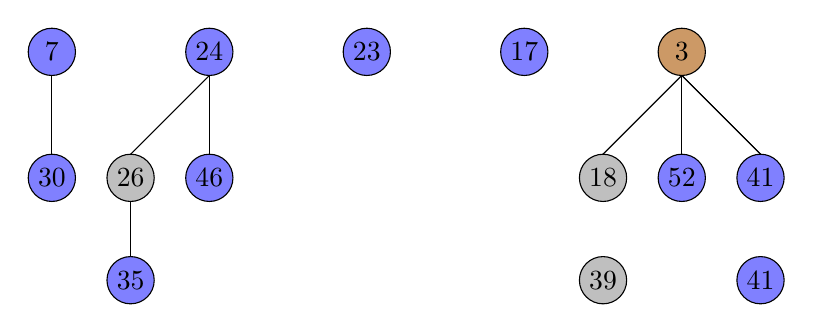
\begin{tikzpicture}
        \draw [fill=blue!50] (0, -7.7) circle (0.3cm) node {7};
        
        \draw [fill=blue!50] (0, -9.3) circle (0.3cm) node {30};
        \draw [fill=blue!50] (2, -9.3) circle (0.3cm) node {46};
        \draw [fill=gray!50] (1, -9.3) circle (0.3cm) node {26}; 
        \draw [fill=blue!50] (1, -10.6) circle (0.3cm) node {35};
        \draw [fill=blue!50] (4, -7.7) circle (0.3cm) node {23};
        \draw [fill=blue!50] (6, -7.7) circle (0.3cm) node {17};
        \draw [fill=blue!50] (2, -7.7) circle (0.3cm) node {24};
        \draw [fill=brown!80] (8, -7.7) circle (0.3cm) node {3};
        \draw [fill=blue!50] (8, -9.3) circle (0.3cm) node {52};
        
        \draw [fill=gray!50] (7, -9.3) circle (0.3cm) node {18};

        \draw [fill=gray!50] (7, -10.6) circle (0.3cm) node {39};
        
        \draw [fill=blue!50] (9, -9.3) circle (0.3cm) node {41};
        \draw [fill=blue!50] (9, -10.6) circle (0.3cm) node {41};
        
        
        \draw (2, -8) -- (2, -9);
        \draw (0, -8) -- (0, -9);
        \draw (2, -8) -- (1, -9);
        \draw (1, -9.6) -- (1, -10.3);
        
        
        
        
        \draw (8, -8) -- (8, -9);
        
        \draw (7, -9) -- (8, -8);
        \draw (9, -9) -- (8, -8);
        \draw (9, -9) -- (8, -8);
        
        
        
    \end{tikzpicture}
\end{frame}

% \begin{frame}{Fibonacci Heap: Extract Mean}
    \begin{tikzpicture}
        \draw [fill=blue!30] (0, -7.7) circle (0.3cm) node {7};
        \draw (0, -8) -- (0, -9);
        \draw [fill=blue!30] (0, -9.3) circle (0.3cm) node {30};
        
        \draw [fill=blue!30] (2, -7.7) circle (0.3cm) node {24};
        \draw (2, -8) -- (2, -9);
        \draw [fill=blue!30] (2, -9.3) circle (0.3cm) node {46};
        \draw [fill=gray!50] (1, -9.3) circle (0.3cm) node {26}; 
        \draw [fill=blue!50] (1, -10.6) circle (0.3cm) node {35}; 
        \draw (2, -8) -- (1, -9);
        \draw (1, -9.6) -- (1, -10.3);
        
        \draw [fill=blue!30] (4, -7.7) circle (0.3cm) node {23};
        \draw [fill=blue!30] (6, -7.7) circle (0.3cm) node {17};
        
        \draw [fill=brown!80] (8, -7.7) circle (0.3cm) node {3};
        \draw (8, -8) -- (8, -9);
        \draw [fill=blue!30] (8, -9.3) circle (0.3cm) node {52};
        
        \draw [fill=gray!50] (7, -9.3) circle (0.3cm) node {18};
        \draw (7, -) -- (8, -9);
        \draw [fill=gray!50] (7, -10.6) circle (0.3cm) node {39};
        
        \draw [fill=blue!30] (9, -9.3) circle (0.3cm) node {41};
        \draw [fill=blue!30] (9, -10.6) circle (0.3cm) node {41};
    \end{tikzpicture}
\end{frame}
\begin{frame}[t]{Fibonacci: text and image}
    \vspace{1cm}
    \begin{columns}[onlytextwidth]
        \column{0.5\textwidth}
            \begin{itemize}
                \item {\color{blue}Extract/delete Min}
                \onslide<2-> {
                    \begin{itemize}
                         \item \alert{Delete} {\color{blue}min} and \alert{add} its {\color{blue}children} into the root list \pause
                         \item {\color{gray}Consolidate trees so that no two roots have same degree}
                    \end{itemize}
                }
            \end{itemize}
        \column{0.5\textwidth}

        \centering
        \only<3-> {
        \begin{figure}
            \includegraphics[scale=0.12]{the-golden-ratio-teaser.jpg}
            \end{figure}
        }
    \end{columns}
\end{frame}

\end{document}